\chapter{Multichroic detectors}
\label{chp:multichroic}

This chapter describes a project to develop arrays of polarization-sensitive, multichroic KID pixels for future CMB experiments.
These detectors are designed to help separate foreground signals from CMB signals by measuring two spectral bands simultaneously.
One band is primarily for detecting the CMB, so it is centered on \SI{150}{GHz}, near the peak of the CMB black body spectrum.
The other band is primarily for detecting Galactic dust signals, so it is centered on \SI{235}{GHz}, where the dust emission is brighter than the CMB.
Some of the material in this chapter was published in \textcite{Johnson2016SPIE} and \textcite{Johnson2017arXiv}.


\section{Overview}
\label{sec:multichroic.overview}

The pixels are each sensitive to two linear polarization states in two spectral bands, so there are four KIDs per pixel.
Each pixel consists of a feedhorn, waveguide, and ortho-mode transducer (OMT) antenna that together couple light from free space onto the chip; microstrip (MS) millimeter-wave circuits that filter and route the light; and four hybrid aluminum-niobium co-planar waveguide (CPW) KIDs that detect the light.
Figure~\ref{fig:multichroic_mkid_coupling_v3} shows drawings of the design.

\begin{figure}[htb]
\centering
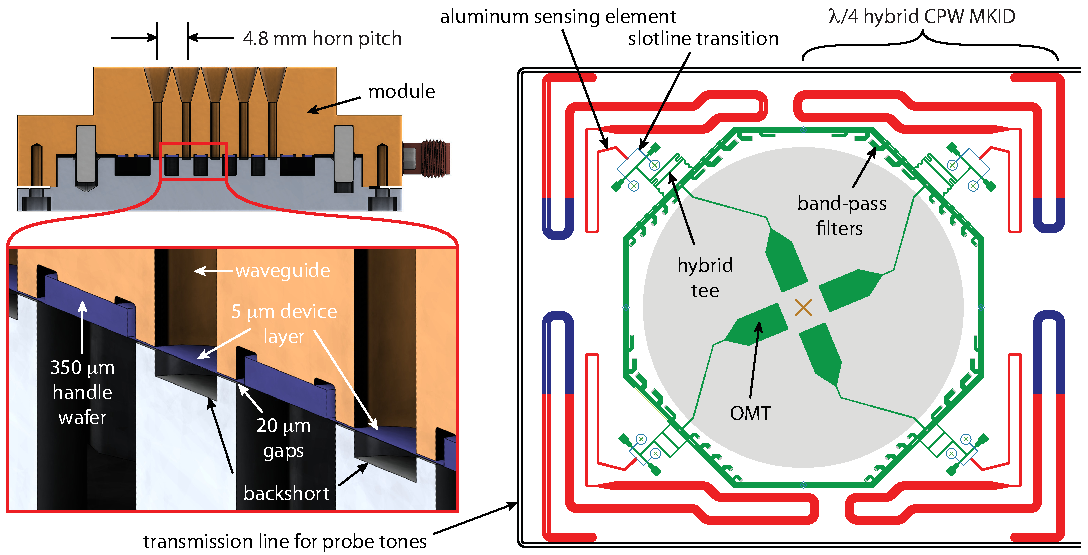
\includegraphics[width=\textwidth]{multichroic/multichroic_mkid_coupling_v3.pdf}
\caption[Drawings of the multichroic detector module and of one multichroic pixel.]
{
\textbf{(Left)}
A drawing of the multichroic detector module.
The upper panel shows a cross-section of the entire module.
The detector wafer (blue) is enclosed between the two aluminum pieces (brown and gray).
Light enters the feedhorns at the top and propagates down the circular waveguide.
The lower panel shows detail of the area where light couples to the OMT antennas, which from this perspective would appear on the underside of the blue membranes.
The bosses that extend the waveguide toward the wafer from both sides form chokes that reduce lateral leakage of light.
The backshorts terminate the waveguides and improve the optical coupling.
\textbf{(Right)}
A drawing of one multichroic pixel.
The two opposing OMT probe pairs (green) in the center of the pixel are sensitive to orthogonal linear polarization states.
The band-pass filters and hybrid (\SI{180}{\degree}) tee, which are microstrip components, create the two spectral bands and combine the signals to select the desired waveguide mode.
The slotline transition couples the light from the microstrip circuitry into the aluminum CPW sensing region of one of the quarter-wavelength CPW KIDs.
The region of the KIDs drawn in red is the same in each pixel, while the region drawn in blue varies in order to set the resonance frequency.
The resonators are weakly coupled to the feedline, shown in gray, by the short lengths (``elbow couplers'') of transmission line that run parallel to it.
This figure was published in \textcite{Johnson2017arXiv}.
}
\label{fig:multichroic_mkid_coupling_v3}
\end{figure}

Our design was based on detectors that were developed for~\autocite{Datta2014JLTP, Henderson2016JLTP, Duff2016JLTP} and deployed on~\autocite{Ho2016JLTP,Datta2016JLTP} the Advanced ACTPol experiment~\autocite{Thornton2016ApJS}, which is a CMB polarization experiment on the Atacama Cosmology Telescope (ACT) in northern Chile~\autocite{ACT2011ApJS}.
Our goal was to replace the bolometers used by ACTPol with KIDs.
For reasons described below, we chose to use silicon-on-insulator (SOI) wafers instead of the dielectrics used in the ACTPol design.
We also chose to replace the ring-loaded ACTPol feedhorns with conical feedhorns, for simplicity of fabrication.
Thus, the initial design tasks were as follows.
First, to re-optimize the feedhorn coupling scheme and millimeter-wave circuitry for SOI.
Second, to develop a circuit to couple the optical radiation from the microstrip circuitry to the KID CPW center strip.
Third, to design and draw CPW resonators with suitable resonance frequencies within the available chip area.
Fourth, to design a metal package to enclose the wafer using the new optical design.
The first two tasks were done by collaborators, and the latter two were primarily my responsibilities.


\section{Optical coupling}
\label{sec:multichroic.optical}

In our prototype design, a conical horn with a \SI{4.66}{mm} diameter aperture and a \SI{15}{\degree} flare angle is used to feed each pixel.
Each horn feeds a \SI{1.49}{mm} diameter circular waveguide that is made approximately \SI{9}{mm} long to ensure that evanescent low-frequency modes do not reach the detectors.
A broadband planar waveguide probe OMT on a thin membrane separates orthogonal linear polarizations.
The orientation of the OMT defines a polarimeter axis that is independent of frequency.
Chokes on both sides of the membrane reduce lateral leakage into the module.
A backshort behind the membrane reflects light that was not absorbed on the first pass, which improves the optical coupling.
Figure~\ref{fig:multichroic_mkid_coupling_v3} shows detail of these structures.

\begin{figure}[htb]
\centering
\includegraphics[width=0.8\textwidth]{multichroic/multichroic_spectral_bands.png}
\caption[Simulations of the spectral bands for the multichroic KID pixels.]
{
Simulations of the spectral bands for the multichroic KID pixels.
This figure was published in \textcite{Johnson2016SPIE}.
}
\label{fig:multichroic_spectral_bands}
\end{figure}

The output of each waveguide probe is CPW, so a broadband CPW-to-MS transition composed of seven alternating sections couples light to the on-chip MS circuitry.
A diplexer consisting of two sets of five-pole resonant-stub MS band-pass filters splits the light into the two spectral bands, \SIrange{125}{170}{GHz} and \SIrange{190}{280}{GHz}.
The results of end-to-end electromagnetic simulations, shown in 
Figure~\ref{fig:multichroic_spectral_bands}, indicate that the expected absorption efficiency is approximately 0.9 across the 150 GHz and the 235 GHz spectral bands.
Circular waveguide supports multiple modes over this fractional bandwidth of 2.25:1, but only the TE$_{11}$ mode has desirable polarization properties.
This mode couples to opposite fins of the OMT with a \SI{180}{\degree} phase shift, while the next highest order mode, which also couples efficiently to the OMT probes, has a \SI{0}{\degree} phase shift.
A \SI{180}{\degree} hybrid combines the light from each probe pair within a single spectral band, and the path lengths from the probes to the inputs of the hybrid are designed to be identical.
To ensure single-mode performance, the sum port of the hybrid is terminated in a resistive gold microstrip, while the difference port is connected to the KID using a broadband coupling circuit that is described below.
To re-optimize the feedhorn coupling and the millimeter-wave circuitry, our collaborators at the University of Michigan performed electromagnetic simulation of the components using ANSYS HFSS software~\autocite{HFSS} and Sonnet EM software~\autocite{Sonnet}. % Jeff McMahon and Rahul Datta

\begin{figure}[htb]
\centering
\includegraphics[width=0.7\textwidth]{multichroic/multichroic_ms-to-cpw_coupler_schematic.png}
\caption[A schematic of the microstrip-to-coplanar-waveguide coupler for the multichroic KID project.]
{
A schematic of the microstrip-to-coplanar-waveguide coupler for the multichroic KID project.
This figure was published in \textcite{Johnson2016SPIE}
}
\label{fig:multichroic_ms-to-cpw_coupler_schematic}
\end{figure}

Our collaborators at Arizona State University designed a MS-to-CPW coupler and optimized it using Sonnet simulations that are described by \textcite{Surdi2016}.  % Philip Mauskopf and Harshad Surdi 
Figure~\ref{fig:multichroic_ms-to-cpw_coupler_schematic} is a schematic of the coupler.
Millimeter-wave light coming from the microstrip output of the \SI{180}{\degree} hybrid is evenly divided in-phase onto two microstrip branches that each have twice the impedance of the input.
Each branch feeds a standard broadband microstrip-to-slotline transition that couples the light into a slotline formed in the ground plane.
The two slotlines come together and meet the CPW gaps in the aluminum section of the MKID.


\section{Prototype resonators: simulation and testing}
\label{sec:multichroic.prototype}

Since the millimeter-wave circuitry required a niobium ground plane, a hybrid KID design was a natural choice.
A hybrid KID is made from two superconductors with different gap energies.
One superconductor, the \textit{active} metal, must have a spectroscopic gap below the photon energy so that optical photons can break pairs in this region of the resonator.
The other superconductor, the \textit{inactive} metal, should have a higher gap so that optically excited quasiparticles in the active region remain trapped there.
In the design presented here, in which optical photons propagate on transmission lines made from the inactive metal, its spectroscopic gap must be higher than the photon energy so that these photons can propagate without loss.
Optically-excited quasiparticles are trapped in the active region since their energies are less than the gap in the inactive metal.

We chose to use CPW resonators with an aluminum active region because hybrid CPW KIDs (using aluminum and niobium-titanium-nitride) have demonstrated excellent sensitivity~\autocite{Yates2011APL,Janssen2013APL,Janssen2014SPIE} and have been incorporated into large arrays~\autocite{Baselmans2017AA}.
The ACTPol OMTs were fabricated on a low-stress silicon nitride (SiN$_x$) membrane formed by etching away the silicon wafer beneath.
Because amorphous dielectrics tend to produce excess loss (Section~\ref{sec:loss.dielectrics}) and noise (Section~\ref{sec:sensitivity.tls}) in KIDs, we decided to avoid using a silicon nitride membrane.
Instead, we planned to use a SOI wafer that consists of a thin crystalline silicon device layer above a thin silicon oxide (SiO$_2$) layer above a thick crystalline silicon handle layer that provides mechanical support.
The membrane would be formed by etching away the dielectrics beneath the device layer.
Lossy dielectrics underneath the KIDs would also be etched away as required.

While transmission-line resonators are a common choice for KIDs, when this project began my group had designed and fabricated only lumped-element resonators.
The starting point for analysis of a CPW resonator is that the structure supports a quasi-transverse electromagnetic (quasi-TEM) mode.
The wave speed $\lightspeed$ for this mode can be approximated using the average dielectric constant of the substrate $\epsilon_\mathrm{substrate}$ and of vacuum~\autocite{Wen1969IEEE}:
\begin{equation}
\lightspeed
  =
  \lsvac \left( \frac{1 + \epsilon_\mathrm{substrate}}{2} \right)^{-1/2},
\end{equation}
where $\lsvac$ is the speed of light in vacuum.
Silicon has dielectric constant $\epsilon = 11.9$ at microwave frequencies.
The length of a quarter-wavelength resonator with a given resonance frequency $\freadout_\resonator$ is thus
\begin{equation}
\tracelength
  =
  \wavelength / 4
  =
  \freadout_\resonator / 4 \lightspeed.
\end{equation}
The wave speed is reduced if the CPW is made from a superconducting structure with significant kinetic inductance, and the resonance frequency shifts accordingly:
\begin{equation}
\freadout_\resonator
  =
  \left(1 - \kifraction \right)^{1/2} \freadout_\resonator(\kifraction = 0).
\end{equation}
\todo[inline]{Discuss calculation of kinetic inductance fraction}
The effective kinetic inductance fraction $\kifraction$ is not trivial to calculate for hybrid resonators.
\textcite{Gao2008} discusses the effective kinetic inductance fraction of superconducting CPW resonators in detail.
\todo[inline]{Use estimates from for center-only and shorted end only}

I used electromagnetic simulations~\autocite{Sonnet} to simulate hybrid quarter-wavelength CPW resonators in order to validate the design and estimate the effective kinetic inductance fraction.
To find the resonance frequencies quickly I used a three-port method~\autocite{Wisbey2014JLTP}, which involves inserting a third port in the CPW center trace where it meets the ground plane, in addition to the two ports on the feedline.
Our heterodyne system can read out resonances up to about \SI{4}{GHz}.
As discussed in Chapter~\ref{chp:theory}, the fractional frequency response is enhanced at lower resonance frequencies, so I targeted frequencies around \SI{3}{GHz}.
In order to achieve the desired resonance frequencies in the limited area that was available, it was necessary to fold the resonators into the shape shown in Figure~\ref{fig:mkidarray01-0101_photo_one_resonator}, which is a photograph of a fabricated resonator.
This exact geometry was too computationally expensive to simulate, but my simulations of simplified resonator geometries indicated that the effective kinetic inductance fraction was around 20\%. 
The simulations also indicated that the participation ratio (see Section~\ref{sec:loss.dielectrics}) of the buried oxide layer was of order 1\%.

\begin{figure}[htb]
\centering
\includegraphics[width=0.8\textwidth]{multichroic/mkidarray01-0101_photo_one_resonator.jpg}
\caption[MKIDArray01-0101: a photograph of one resonator.]
{
MKIDArray01-0101: a photograph of one resonator, showing the area available in one corner of a pixel.
The ground plane appears green, and the exposed silicon is gray.
The orange structure is silicon nitride that is used for the microstrip circuitry and is removed from around the KIDs.
The horizontal transmission line that crosses the photograph is the feedline.
The area below the photo border is occupied by another resonator in the same pixel, and the area to the right of the photo border is occupied by a resonator in the adjacent pixel.
Photo courtesy of Brad Johnson.
}
\label{fig:mkidarray01-0101_photo_one_resonator}
\end{figure}

Using input from the simulations, I drew and tested prototype CPW resonators in order to explore resonator designs and provide feedback to collaborators on fabrication issues such as film quality.
Figure~\ref{fig:multichroic_prototypes} shows a drawing of a chip with eight CPW resonators and a photograph of a small aluminum package I designed that containing a chip fabricated by our colleagues at Stanford University. % Sherry Cho and Dale Li 
All of the prototype resonators consisted of either one or two films on high-resistivity, float-zone silicon substrates, so they involved a small number of fabrication steps.

\begin{figure}[htb]
\centering
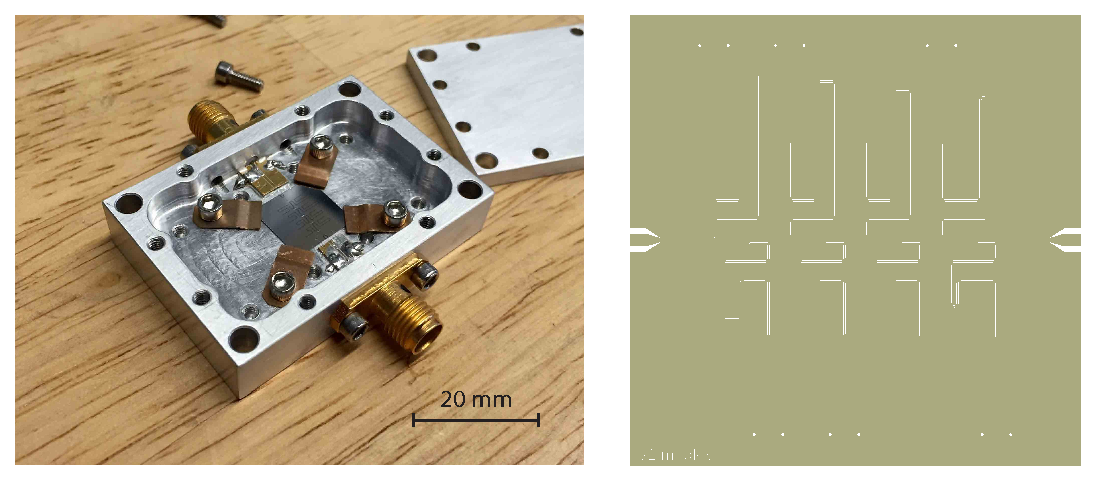
\includegraphics[width=\textwidth]{multichroic/multichroic_prototypes.pdf}
\caption[A photograph and a drawing of a chip with eight prototype resonators.]
{
\textbf{(Left)}
A photograph of a chip with eight prototype CPW KIDs in a small aluminum package designed for dark testing.
\textbf{(Right)}
A drawing of an eight-resonator chip that contains four different resonator types that are designed to test different aspects of the design.
The tan area is niobium, the red area is aluminum, and the white areas are exposed substrate.
This figure was published in \textcite{Johnson2016SPIE}.
}
\label{fig:multichroic_prototypes}
\end{figure}

Some tests were performed in a cryostat that had no magnetic shielding, and early generations of prototype resonators had high internal loss.
After we recognized that the magnetic shielding was insufficient, we obtained sheets of a nickel-iron-cobalt alloy (similar to mu-metal) and formed them by hand into a small box with end caps.
We tested the next generation of all-niobium resonators inside this box.
While this material had not been validated for cryogenic use, we obtained much lower internal loss
$\loss_\internal \sim \num{2.5e-6} = 1 / (\num{4e5})$.
This result suggested that vortices had caused some of the loss in previous generations of resonators.

The simulations and prototype resonators included the slot structures on the ground plane layer of the MS-to-CPW coupler, which are visible in Figure~\ref{fig:multichroic_prototypes}.
Our conclusion from simulations and measurements was that the slotline sections, which are electrically short at the KID resonance frequencies, did not have a significant effect on the resonators.

The initial KID design called for the active region to consist of a \SI{40}{nm} strip of aluminum deposited on top of the \SI{200}{nm} niobium ground plane layer.
To ensure continuity of the aluminum, the plan was to use a niobium etch that produced a sloped transition between the top of the niobium and the exposed silicon.
Due to difficulties in developing a high-yield fabrication process for the aluminum-over-niobium design, we explored a new fabrication process.
This niobium-over-aluminum process involved first depositing the aluminum followed immediately by the niobium without breaking vacuum, to avoid oxide formation.
Then, the niobium was etched from the CPW gaps and from the active region.
Finally, the aluminum was etched from the CPW gaps.
The resulting structure consists of a niobium-aluminum bilayer everywhere except for the active region, which is only aluminum.
Despite the continuity of the aluminum, the gap energy in the aluminum underneath the niobium should be significantly elevated due to the proximity effect, and the structure is expected to trap quasiparticles in the active region.
Prototype niobium-over-aluminum resonators had high loss under dark conditions, typically
$\num{2.5e-5} < \loss_\internal < \num{2e-4}$,
corresponding to 
$\num{40000} > \qf_\internal > \num{5000}$.
We have not yet been able to determine whether this loss is due to vortices, to the fabrication process, or to effects inherent to the bilayer.
The two 23-pixel wafers described below were fabricated with niobium-over-aluminum bilayers.


\section{The 23-pixel design}
\label{sec:multichroic.23-pixel}

Our collaborators at Stanford University used the structures resulting from the electromagnetic simulations and arranged them to produce a layout for the millimeter-wave circuitry. % Sherry Cho, Dale Li, and Yanru Song 
Using input from my simulations and from the prototype resonators, I designed 92 KID resonators and a feedline to add to this layout.
Figure~\ref{fig:multichroic_23-pixel_layout} is a drawing of the resulting 23-pixel design.

\begin{figure}[htb]
\centering
\includegraphics[width=0.7\textwidth]{multichroic/multichroic_23-pixel_layout.pdf}
\caption[A drawing of the multichroic 23-pixel array.]
{
A drawing of the multichroic 23-pixel array.
The pixel centers are separated by \SI{4.8}{mm} and the chip is approximately \SI{30}{mm} on each side.
There are two pixel polarization axes that differ by \SI{45}{\degree} and alternate along the rows.
The feedline meanders between the pixels and is connected to external transmission lines using the bond pads at right.
The four gray ovals are alignment slots that are etched in the silicon.
Precisely machined bosses on the holder protrude into these slots and align the chip to within about \SI{10}{\micro\meter}, while allowing for differential thermal contraction between the silicon and aluminum.
%See Appendix~\ref{chp:hardware}.
}
\label{fig:multichroic_23-pixel_layout}
\end{figure}

Each KID on a given feedline requires a unique resonance frequency, so some part of each KID must be unique.
The chips containing eight prototype resonators had a square footprint \SI{10}{mm} on a side, which could be flashed using a single photomask.
In order to fabricate the much larger 23-pixel (92-resonator) array using a reasonable number of photomasks, we fixed the lengths of the active regions and set each resonance frequency by tuning the length of the inactive region using a ``trombone slide'' structure.
In both Figure~\ref{fig:multichroic_mkid_coupling_v3} and Figure~\ref{fig:multichroic_23-pixel_layout}, the KIDs are drawn in both red and blue.
The red areas are identical between all pixels, while the blue areas vary between pixels because the trombone slide overlaps the fixed region by different amounts and produces a different total length for each KID.

The geometry of the active CPW section was determined based on both the simulations of the MS-to-CPW coupling and on simulations that indicated that nearly all of the millimeter wave light would be absorbed over a length of about \SI{2}{mm}.
The aluminum center strip in the active region is \SI{4}{\micro\meter} wide, and the gaps to the niobium-over aluminum ground plane are \SI{5}{\micro\meter} wide.
The active region is \SI{2.1}{mm} long for the \SI{150}{GHz} detectors and is \SI{2.7}{mm} long for the \SI{235}{GHz} detectors.
The aluminum strip is longer for the \SI{235}{GHz} detectors because we anticipate they will receive more power from the sky, so their volume needs to be larger to maintain equal dissipation.
The geometry of the inactive section, made from the niobium-over-aluminum bilayer, has a length range of \SIrange{8.8}{10.4}{mm}.
The end of the resonator near the readout transmission line supports the largest electric fields and is therefore most susceptible to TLS effects~\autocite{Gao2008aAPL, Gao2008bAPL,Zmuidzinas2012ARCMP}.
To reduce these effects, the inactive center strip is \SI{10}{\micro\meter} wide and the gaps to the ground plane are \SI{30}{\micro\meter} wide.
The geometry of the elbow coupler that runs along the transmission line is the same as the rest of the inactive CPW.
The feedline is CPW with a \SI{20}{\micro\meter} center strip and \SI{12}{\micro\meter} gaps to the ground plane.
It is designed to match the \SI{50}{\Omega} impedance of the boards that carry signals to and from the coaxial connectors and the chip.

The exact lengths were calculated for each resonator assuming the effective dielectric constant discussed above and an effective kinetic inductance fraction of 20\% for all resonators, which is an approximation.
Because the \SI{235}{GHz} detectors have longer active sections, their inactive sections are proportionally longer, and they have lower resonance frequencies than the \SI{150}{GHz} detectors.
The low-frequency \SI{235}{GHz} detectors are in the lower left of each pixel, and their resonance frequencies span \SIrange{2542}{2634}{MHz}.
The high-frequency \SI{235}{GHz} detectors are in the lower right of each pixel, and their resonance frequencies span \SIrange{2664}{2756}{MHz}.
The low-frequency \SI{150}{GHz} detectors are in the upper right of each pixel, and their resonance frequencies span \SIrange{2786}{2878}{MHz}.
The high-frequency \SI{150}{GHz} detectors are in the upper left of each pixel, and their resonance frequencies span \SIrange{2908}{3000}{GHz}.
The bands were separated by \SI{30}{MHz} in order to reduce frequency collisions.
The total bandwidth of about \SI{460}{MHz} allows all 92 resonators in the array to be read out simultaneously using our heterodyne system if the local oscillator frequency is placed between the two middle bands.

\begin{table}[htb]
\centering
\footnotesize
\caption[The stack-up for the first multichroic detector array on a SOI wafer.]
{
The stack-up for the first multichroic detector array on a SOI wafer.
The direction of light propagation is from the bottom of the table to the top.
Because the thick silicon handle wafer and silicon oxide layer are etched away from under the OMTs, the light first encounters the thin silicon device layer.
HTO: hot thermal oxide.
}
\renewcommand{\arraystretch}{1.2}
\begin{tabular}{c d{2} l}
\toprule
Material & \mathrm{Thickness} / \si{\micro m} & Notes \\
\midrule
Al & \mathrm{bulk} & lid with back-shorts \\
vacuum & \mathrm{varies} & from metal on wafer to package bulk metal \\
\midrule
Au & 0.1 & \SI{180}{\degree} tee termination and heat sink wirebond pads \\
Nb & 0.4 & microstrip: filters, hybrids, coupler; feedline cross-overs \\
SiN$_x$ & 0.35 & not present above the resonators or feedline \\
Nb & 0.2 & ground plane: resonators, feedline, OMTs \\
Al & 0.04 & ground plane and KID active region \\
\midrule
Si (intrinsic $\langle 100 \rangle$) & 5 & resistivity $>\SI{e4}{\ohm.cm}$, float-zone; thickness $\pm \SI{0.5}{\micro m}$ \\
SiO$_2$ (wet HTO) & 0.5 & thickness $\pm 5\%$ \\
Si (P / boron $\langle 100 \rangle$) & 350 & resistivity \SIrange{1}{10}{\ohm.cm}; thickness $\pm \SI{5}{\micro m}$ \\
\hline
Al & \mathrm{bulk} & holder with feedhorns and circular waveguides \\
\bottomrule
\end{tabular}
\label{tab:multichroic_stack-up}
\end{table}


\section{Fabrication}
\label{sec:multichroic.fabrication}

All of the arrays were fabricated by our collaborators at Stanford University.
The first 23-pixel KID array was fabricated on SOI wafers \SI{100}{mm} in diameter.
Each SOI wafer consists of a \SI{5}{\micro\meter} thick float-zone silicon (> \SI{10}{k\Omega.cm} resistivity) device layer and a \SI{350}{\micro\meter} thick silicon handle wafer held together by a \SI{0.5}{\micro\meter} thick buried oxide layer.
An aluminum-niobium bilayer is first deposited on the device layer.
The aluminum is \SI{40}{nm} thick and the niobium is \SI{200}{nm} thick.
This bilayer forms the ground plane, and is patterned to produce the OMTs, some millimeter-wave circuitry, the coupler slotlines and KIDs, and the feedline.
A \SI{350}{nm} thick film of silicon nitride (SiN$_x$) is deposited on top of the bilayer, followed by a \SI{400}{nm} thick niobium film.
The silicon nitride serves as the electrically insulating dielectric material in the microstrip, and the niobium film is patterned to form the microstrip circuit that includes the band-pass filters and the \SI{180}{\degree} hybrids.
Our design uses cross-unders~\autocite{Duff2016JLTP} in the microstrip circuit rather than cross-overs, which decreases the number of required fabrication steps.
A gold film is deposited and patterned on top of the silicon nitride to construct the termination resistor at the sum port of the \SI{180}{\degree} hybrid.
The silicon nitride is removed near the KIDs to reduce loss and two-level system noise.
The niobium is removed from the approximately \SI{2}{mm} long sensing section of the center line of the KIDs, leaving only the aluminum.
To form the membrane and alignment slots, the thick silicon handle wafer is removed using deep reactive ion etching (DRIE), and the buried oxide layer is then removed using hydrogen fluoride (HF) vapor.
To reduce TLS noise and loss, these dielectrics are also removed from underneath the high-field section of the KIDs.
Table~\ref{tab:multichroic_stack-up} summarizes the fabrication stack-up.


\section{MKIDArray01-0101: a 23-pixel array on intrinsic silicon}
\label{sec:multichroic.mkidarray01}

In order to test fabrication steps and the resonator design, we produced an engineering array on a monolithic \SI{500}{\micro\meter} thick high-resistivity, float-zone silicon wafer.
This engineering wafer, which we called MKIDArray01, was not optimized for millimeter-wave coupling because the substrate was too thick.
I tested chip 0101 from this wafer in a simplified version of the aluminum horn package with no horns, chokes, or backshorts.
Figure~\ref{fig:mkidarray01_in_dark_and_horn} shows a photograph of this array in a dark holder, as well as a holder with conical horns that was used later on for optical testing.
The package was enclosed in a box made from magnetic shielding material.

\begin{figure}[htb]
\centering
\includegraphics[width=\textwidth]{multichroic/mkidarray01_in_dark_and_horn.pdf}
\caption[Photographs of the holder, showing the conical horns, and of MKIDArray01-0101 in a dark holder.]
{
Photographs of the holder, showing the conical horns, and of MKIDArray01-0101 in a dark holder.
}
\label{fig:mkidarray01_in_dark_and_horn}
\end{figure}

Figure~\ref{fig:mkidarray01_full_s21_sweep} shows the result of sweeping readout tones from \SIrange{1.8}{4.0}{GHz} and recording the complex forward scattering parameter $\forwardscattering$.
All 92 designed resonances seemed to be present, along with some additional resonances that did not respond much to temperature changes and thus could be box modes or resonances involving the ground plane.
The KID resonances appeared slightly above the nominal resonance frequencies, indicating that the effective kinetic inductance fractions were slightly less than the 20\% estimate used to calculate the resonator lengths.

The scatter in the measured resonance frequencies, apparent in the frequency sweep, is due to a known effect.
The elbow coupler radiates onto the feedline both the quasi-TEM mode, in which the ground planes have the same voltage, and a so-called slotline mode, in which the ground plane voltages are different.
The slotline mode can be trapped on the chip and develop standing waves, which affect both the coupling strength and the location of the resonance frequency.
This effect can be mitigated by electrically connecting the ground planes of the CPW~\autocite{Mates2011, Yates2014JLTP}.
We designed cross-overs to address this issue, but did not include them in the photomask set used for the wafers described in this thesis because the fabrication process was not yet developed.

\begin{figure}[htb]
\centering
\includegraphics[width=\textwidth]{multichroic/mkidarray01_full_s21_sweep.pdf}
\caption[MKIDArray01-0101: a wide frequency sweep showing many resonance dips.]
{
MKIDArray01-0101: a wide frequency sweep showing many resonance dips.
The vertical gray lines show the nominal resonance frequencies.
}
\label{fig:mkidarray01_full_s21_sweep}
\end{figure}

We fit the resonances identified in the frequency sweep to the model given in Section~\ref{sec:theory.resonator} to determine the internal and coupling quality factors for many of the resonators on the array.
Figure~\ref{fig:mkidarray01_histogram_Qi_Qc} shows a histogram of the result.
The coupling quality factors show wide scatter that is expected in the absence of cross-overs.
The internal quality factors are clustered just below
$\qf_\internal \sim \num{20000}$,
corresponding to
$\loss_\internal \sim \num{5e-5}$.
Although the magnetic shielding has improved, the loss values are similar to those obtained in the prototype niobium-over-aluminum resonators, suggesting that vortices are not dominating the loss.
The internal loss was nearly independent of readout power, so TLS loss is unlikely to be significant. 

\begin{figure}[htb]
\centering
\includegraphics[width=0.5\textwidth]{multichroic/mkidarray01_histogram_Qi_Qc.pdf}
\caption[MKIDArray01-0101: a histogram of resonator quality factors.]
{
MKIDArray01-0101: a histogram of resonator quality factors.
}
\label{fig:mkidarray01_histogram_Qi_Qc}
\end{figure}

The response of seven resonators to varying bath temperature is shown in Figure~\ref{fig:mkidarray01_seven_s_and_i_vs_temperature}.
The central five resonators respond qualitatively as expected for resonators containing aluminum.
The leftmost and rightmost resonators, which seem not to be KIDs, barely respond to the temperature change.

\begin{figure}[htb]
\centering
\includegraphics[width=\textwidth]{multichroic/mkidarray01_seven_s_and_i_vs_temperature.pdf}
\caption[MKIDArray01-0101: response to changing bath temperature for seven resonators.]
{
MKIDArray01-0101: response to changing bath temperature for seven resonators.
The left axes all share the same limits, and show internal loss $\loss_\internal$.
The right axes all share the same limits, which are much larger, and show the fractional frequency shift
$\shift(\temperature)$
from the maximum measured resonance frequency $\freadout_\resonator^\mathrm{max}$.
}
\label{fig:mkidarray01_seven_s_and_i_vs_temperature}
\end{figure}

The critical temperature was measured to be, using the through transmission on the bilayer feedline, $\tc = \SI{8.3}{K}$, somewhat reduced from the value of \SI{9.3}{K} for bulk niobium.
The resonators become too lossy to measure as the chip temperature approaches the critical temperature of aluminum, so the aluminum film transition temperature is unknown.


\section{MKIDArray02-0001: a 23-pixel array on SOI}
\label{sec:multichroic.mkidarray02}

\begin{figure}[htb]
\centering
\includegraphics[width=0.5\textwidth]{multichroic/MKIDArray02-0001_in_package.jpg}
\caption[MKIDArray02-0001: a photograph of the first 23-pixel chip on a silicon-on-insulator wafer.]
{
MKIDArray02-0001: a photograph of the first 23-pixel chip on a silicon-on-insulator wafer in a package I designed for optical testing.
Photo courtesy of Brad Johnson.
}
\label{fig:MKIDArray02-0001_photo}
\end{figure}

This wafer, which we called MKIDArray02, was the first to be fabricated using SOI.
I tested one 23-pixel chip from this wafer, number 0001.
The dielectrics were removed from underneath the elbow couplers, which is the area of highest electric field.
Figure~\ref{fig:starcryo_cryostat_with_hwp} is a photograph of the cryostat that shows the experimental configuration and the optical components I used to illuminate the detectors.
I used both the Eccosorb black body source and the electronic millimeter-wave source for these first optical tests.
Figure~\ref{fig:mkidarray02_wide_sweep_180_mK_real_and_fake} shows wide frequency sweeps at two temperatures, which were used to distinguish between KIDs and spurious resonances.
I was able to identify 66 of the 92 expected KID resonances, as well as a number of additional resonances that do not seem to be KIDs.

\begin{figure}[htb]
\centering
\includegraphics[width=0.8\textwidth]{multichroic/mkidarray02_wide_sweep_180_mK_real_and_fake.pdf}
\caption[MKIDArray02-0001: wide frequency sweeps at two temperatures.]
{
MKIDArray02-0001: wide frequency sweeps at two temperatures.
The red data points were acquired with the package temperature at \SI{0.2}{K}, while the blue data points were acquired at \SI{0.8}{K}.
Aluminum is relatively lossy at the higher temperature, so resonances that produce a transmission dip at this temperature must not be KIDs.
The gray vertical lines show the nominal resonance frequencies.
The brown vertical lines show the frequencies of spurious resonances that remained at the higher temperature.
The green vertical lines show the frequencies of resonances that vanished at the higher temperature and are thus likely to be KIDs.
}
\label{fig:mkidarray02_wide_sweep_180_mK_real_and_fake}
\end{figure}

I measured in detail a subset of 34 resonances, several of which subsequently turned out not to be KIDs.
Data from these resonances is shown in Figures~\ref{fig:mkidarray02_all_scans_Qi_and_Qc_vs_frequency},~\ref{fig:mkidarray02_all_bath_temperature_response},~\ref{fig:mkidarray02_loss_i_and_loss_c_versus_readout_power}, and~\ref{fig:mkidarray02_all_eccosorb_response}.
In some cases, data cuts reduced the number of analyzed resonators below 34.

\begin{figure}[htb]
\centering
\includegraphics[width=0.7\textwidth]{multichroic/mkidarray02_all_scans_Qi_and_Qc_vs_frequency.pdf}
\caption[MKIDArray02-0001: $\qf_\internal$ and $\qf_\coupling$ versus frequency.]
{
MKIDArray02-0001: $\qf_\internal$ and $\qf_\coupling$ versus frequency.
}
\label{fig:mkidarray02_all_scans_Qi_and_Qc_vs_frequency}
\end{figure}

Figure~\ref{fig:mkidarray02_all_scans_Qi_and_Qc_vs_frequency} shows the quality factors extracted from fitting this group of resonances at a bath temperature of \SI{0.19}{K}, which was used for most data collection.
(Due to a cryogenic problem, I used a somewhat higher bath temperature than normal.)
Many of the the other resonances were very shallow or were difficult to analyze due to frequency collisions.
The internal quality factors are similar to those found on the engineering array.
The coupling quality factors are several times higher than on the engineering array, probably because the removal of the dielectrics under the elbow coupler reduces the capacitance between it and the feedline.
The coupling strength can easily be increased by lengthening the section of elbow coupler parallel to the feedline or by moving it closer to the feedline.
The combination of low coupling strength and high internal loss makes the resonances wide and shallow, mostly less than \SI{1}{dB} deep.
Such resonances are difficult to distinguish from the ripple in the background transmission.
It is thus likely that more resonances are present than I was able to identify.

\begin{figure}[htb]
\centering
\includegraphics[width=0.8\textwidth]{multichroic/mkidarray02_all_bath_temperature_response.pdf}
\caption[MKIDArray02-0001: response to changing bath temperature.]
{
MKIDArray02-0001: response to changing bath temperature.
The minimum value of the internal loss for each detector has been subtracted, and the left axis shows the change in loss.
The right axis shows fractional frequency shift $\shift$.
}
\label{fig:mkidarray02_all_bath_temperature_response}
\end{figure}

Measurements of the response of the same 34 resonators to changing bath temperature are shown in Figure~\ref{fig:mkidarray02_all_bath_temperature_response}.
At high temperatures, both $\loss_\internal$ and $\shift$ increase with increasing temperature, as expected.
The low-temperature increase in $\shift$ as the temperature decreases is a signature of TLS effects, and is sometimes called ``back-bending.''

\begin{figure}[htb]
\centering
\includegraphics[width=0.8\textwidth]{multichroic/mkidarray02_loss_i_and_loss_c_versus_readout_power.pdf}
\caption[MKIDArray02-0001: response to changing readout power.]
{
MKIDArray02-0001: response to changing readout power.
The left plot shows internal loss, and the right plot shows coupling loss.
}
\label{fig:mkidarray02_loss_i_and_loss_c_versus_readout_power}
\end{figure}

Figure~\ref{fig:mkidarray02_loss_i_and_loss_c_versus_readout_power} shows the response of the internal and coupling loss to changing readout power.
The observed decrease in $\loss_\internal$ with increasing readout power is a signature of TLS loss.
This occurs because the TLS become saturated~\autocite{Zmuidzinas2012ARCMP}.
\todo[inline]{Backbending in Budoyo2016PRB?}
%However, similar behavior has also been attributed to nonequilibrium effects caused by the readout~\autocite{Budoyo2016PRB}.
Because the internal loss of the resonators fabricated on intrinsic silicon was nearly independent of readout power, the buried oxide layer in this array is the likely culprit.
As usual, the coupling strength $\loss_\coupling$ is independent of readout power.

\begin{figure}[htb]
\centering
\includegraphics[width=0.8\textwidth]{multichroic/mkidarray02_all_eccosorb_response.pdf}
\caption[MKIDArray02-0001: response to changing black body temperature.]
{
MKIDArray02-0001: response of 29 resonators to changing black body temperature.

}
\label{fig:mkidarray02_all_eccosorb_response}
\end{figure}

I tested the response of the same set of detectors to a change in the temperature of a black body load.
This load is the slab of Eccosorb, a material that is black at millimeter wavelengths, that is shown in Figure~\ref{fig:starcryo_cryostat_with_hwp}.
The thickness is such that the slab is nearly opaque, and the transverse extent is sufficient to fill the detector feed horn beams.
The slab has an anti-reflection coating of etched Teflon.
I measured the resonators with the black body at \SI{3.3}{K}, the base temperature of the slab, and at \SI{5.0}{K}, heating the slab using a resistor attached to the slab support structure.
The changes in the internal loss and coupling loss are shown in Figure~\ref{fig:mkidarray02_all_eccosorb_response}.
The brown vertical lines mark the locations of the spurious resonances that were identified later.
These resonances respond either anomalously or not at all the the black body.
The identified KID resonances mostly shift similarly, with the fractional frequency shift $\shift = \delta \freadout_\resonator / \freadout_\resonator$ somewhat higher than the internal loss shift $\delta \loss_\internal$, as expected.
The fractional frequency shift is about 4 parts per million per degree kelvin.

% Chosen one
I chose one resonator to analyze in more detail.
This resonator has a resonance frequency 
$\freadout_\resonator = \SI{3410}{MHz}$
and it is thus likely to be a \SI{150}{GHz} detector.
The internal loss and coupling loss are
\begin{align}
\loss_\internal &= \num{8.14e-5} = 1 / (\num{1.23e4}) \\
\loss_\coupling &= \num{1.92e-5} = 1 / (\num{5.22e4}).
\end{align}
This internal loss is typical for the array, while the coupling loss is lower than average, which makes the resonance deeper and easier to measure.
The resonator bandwidth is
\begin{equation}
\faudio_\resonator
  =
  \freadout_\resonator (\loss_\internal + \loss_\coupling) / 2
  = 
  \SI{170}{kHz},
\end{equation}
which is higher than the Nyquist frequency of \SI{125}{kHz}.
The quasiparticle relaxation time was extracted under similar conditions from the fit in Figure~\ref{fig:mkidarray02_chosen_one_x_fold_fit}, and the  corresponding quasiparticle bandwidth is
$\faudio_\quasiparticle
  =
  1 / (2 \pi \qprelaxationtime)
  =
  \SI{920}{Hz}$.
Figure~\ref{fig:mkidarray02_chosen_one_di_and_s_versus_temperature} shows the response of this resonator to changing bath temperature.
The interpretation of the results is complicated by what appear to be TLS effects on both the internal loss and fractional frequency shift.

\begin{figure}[htb]
\centering
\includegraphics[width=0.8\textwidth]{multichroic/mkidarray02_chosen_one_noise_spectra.pdf}
\caption[MKIDArray02-0001: noise spectra for the \SI{3410}{MHz} resonator.]
{
MKIDArray02-0001: noise spectra for the \SI{3410}{MHz} resonator.
The plotted data are estimates of the power spectral densities of $\detuning(\time)$ and $\loss_\internal(\time)$ extracted from \SI{33}{s} of time-ordered data.
The normalization of the internal loss spectrum is chosen so that the amplifier noise has the same amplitude in both spectral densities.
The roll-off at the highest frequencies is due to an anti-aliasing filter in the readout firmware.
}
\label{fig:mkidarray02_chosen_one_noise_spectra}
\end{figure}

Figure~\ref{fig:mkidarray02_chosen_one_noise_spectra} shows noise data measured at a bath temperature of \SI{0.16}{K} with no optical illumination except for the black body at its \SI{3.3}{K} base temperature.
The spectral density $\spectraldensity_{\loss_\internal \loss_\internal}$ of the internal loss data falls off rapidly below \SI{100}{Hz} to the amplifier noise level and is then white out to the roll-off due to an anti-aliasing filter.
The temperature regulation was particularly unstable in this cooldown, and the stage temperature often fluctuated by up to \SI{1}{mK}, much more than normal.
Some of the noise is thus likely to be produced by changes in the thermal quasiparticle generation rate.
The excess seen in the spectral density $\spectraldensity_{\detuning \detuning}$ of the detuning data may be caused by TLS noise, but more tests would be required to determine the different contributions.

\begin{figure}[htb]
\centering
\includegraphics[width=\textwidth]{multichroic/mkidarray02_chosen_one_mmw_decimated_and_folded.pdf}
\caption[MKIDArray02-0001: decimated and folded time-ordered data for the \SI{3410}{MHz} resonator.]
{
\textbf{(Left)}
Time-ordered detuning data from the \SI{3410}{MHz} resonator.
One time series was taken with the millimeter-wave source off.
The other was taken with the signal chopped at \SI{122}{Hz} using a switch in the source.
Both time series have been decimated by a factor of 64 to remove high-frequency amplifier noise.
\textbf{(Right)}
The entire \SI{33}{s} time series of chopped data, part of which is shown in the left panel, has been folded down to a single period by averaging all samples that are separated by one period.
}
\label{fig:mkidarray02_chosen_one_mmw_decimated_and_folded}
\end{figure}

Figure~\ref{fig:mkidarray02_chosen_one_mmw_decimated_and_folded} shows the response of this detector to a chopped signal from the millimeter wave source described in Section~\ref{sec:sensitivity.measuring} and in Appendix~\ref{chp:hardware}.
The source was used in broadband mode, producing a chaotic  signal from \SIrange{140}{160}{GHz}.
Comparing the data to the black body response indicates that the source signal amplitude corresponds to about a \SI{1}{K} change.
The decay portion of the data shown in the right panel was used for the fit shown in Figure~\ref{fig:mkidarray02_chosen_one_x_fold_fit}.

\begin{figure}[htb]
\centering
\includegraphics[width=0.8\textwidth]{multichroic/mkidarray02_chosen_one_fit_hwp.pdf}
\caption[MKIDArray02-0001: half-wave plate data for the \SI{3410}{MHz} resonator.]
{
MKIDArray02-0001: half-wave plate data for the \SI{3410}{MHz} resonator.
Each blue point is the peak-to-peak amplitude of the time-ordered detuning data at that HWP angle with the source chopped at \SI{122}{Hz}, with statistical error bars.
The amplitude was calculated from about \SI{1}{s} of time-ordered data that was folded to a single period of the chop signal, as in the right panel of Figure~\ref{fig:mkidarray02_chosen_one_mmw_decimated_and_folded}.
The red line is a fit to an offset sine with a period of one quarter HWP rotation, which is the expected modulation period.
}
\label{fig:mkidarray02_chosen_one_fit_hwp}
\end{figure}

I made preliminary measurements of the polarization response of the detectors using the cryogenic sapphire half-wave plate (HWP) shown in Figure~\ref{fig:starcryo_cryostat_with_hwp}.
The HWP was rotated using a cryogenic motor.
Data taken at 100 different HWP angles, corresponding to a full rotation, is shown in Figure~\ref{fig:mkidarray02_chosen_one_fit_hwp}.
The temperature regulation ended halfway through data acquisition and the stage warmed by about \SI{50}{mK} by the end.
The increased thermal quasiparticle density is the likely cause of the decrease in response toward the right of the plot.
Nevertheless, the modulation period of one quarter rotation matches expectations.
The modulation depth is about 50\%, where one would expect 100\% for a perfectly linearly polarized signal measured by an ideal detector.
This may be caused by non-ideal aspects of either the light illuminating the detectors or the detectors themselves, and these possibilities are not mutually exclusive.
First, the illumination may not be perfectly linear.
The HWP acts ideally only at a single frequency close to \SI{150}{GHz}.
As the optical frequency departs from this the polarization will become elliptical, and an ideal detector will measure cross-polarization.
The horn apertures in the package may not be in the far field of the waveguide horn that illuminates them, they are not illuminated perfectly on-axis, and reflections in the optical system complicate analysis.
Second, even if the incoming signal and polarization analyzer were ideal, crosstalk between detectors could also reduce the modulation depth.
The resonators are designed so that nearest neighbors in frequency are separated by at least the pixel-to-pixel spacing of \SI{4.8}{mm}, and the CPW ground plane strongly confines the fields, so direct electromagnetic coupling is unlikely to be significant.
Independent of the physical spacing, resonators that are spaced too closely in frequency compared to their bandwidth will couple to each other through the feedline.
The relatively high internal loss on this array produces low total resonator quality factors and thus wider resonator bandwidths.
Crosstalk may be significantly reduced by connecting the ground planes of the CPW feedline~\autocite{Yates2014JLTP}, which was not done on this chip.
The chokes shown in Figure~\ref{fig:multichroic_mkid_coupling_v3} are designed to suppress light leakage into the module cavities, which could cause incoming signals to illuminate several KIDs on a pixel.
Propagation of substrate modes can be mitigated by using a superconducting mesh with a lower gap than the sensing metal~\autocite{McCarrick2016JLTP, Baselmans2017AA}.
Such a mesh will also reduce crosstalk due to phonons produced by pair recombination, which can propagate significant distances across a chip~\autocite{Patel2017PRB}.


\section{Conclusions and future work}
\label{sec:multichroic:future}

The encouraging results of these first optical tests validate the basic design.
They demonstrate that the millimeter-wave circuitry -- including the MS-to-CPW coupler, which we had not previously tested -- can couple light from the waveguide into the KIDs, that the KIDs respond to light, and that the pixels have some ability to discriminate between linear polarization states.

Adding the ground plane straps should improve the uniformity of the resonance frequency spacing, reduce scatter in the coupling quality factors, and reduce crosstalk.
The coupling strength may be increased to better match the internal loss by lengthening the elbow couplers or by bringing them closer to the feedline. 
If TLS effects are indeed significant, they may be mitigated by removing more of the dielectrics from beneath the resonators.
The source of the loss that limits the internal quality factors may be investigated further both by fabricating more resonators using bilayer films and by comparing the internal loss between resonators fabricated on SOI wafers and on intrinsic silicon wafers.
Future tests with a millimeter-wave source for the \SI{235}{GHz} band will test the spectral discrimination.

Straightforward improvements in the experimental setup, in the pixel design, and in fabrication could lead to a deployment-quality detector array.
Figure~\ref{fig:multichroic_hex_array} shows a concept drawing of a 169-pixel (676-KID) array of these multichroic pixels that could be used in future CMB polarization experiments.


\begin{figure}[htb]
\centering
\includegraphics[width=0.8\textwidth]{multichroic/multichroic_hex_array.png}
\caption[A drawing of a prototype 169-pixel multichroic detector array.]
{
A drawing of a prototype 169-pixel multichroic detector array.
}
\label{fig:multichroic_hex_array}
\end{figure}
